Voor de navigatie is het voldoende om het nieuwe project aan te maken. 
Hierbij zit de navigatie al geïmplemnteerd.

\paragraph{1. Gradle instellingen aanpassen}
Om de SplashScreen API te gebruiken, moeten deze aan de dependacies worden toegevoegd. Dit wordt gedaan in
het \textbf{build.gradle(module)} bestand.
\begin{minted}{kotlin}
dependencies {
    // andere dependacies
    implementation("androidx.core:core-splashscreen:1.0.0")
}
\end{minted}

\paragraph{2. SplashScreen instellen}
Na het toevoegen van de dependancy kan het laadscherm aangepast worden. 
Hiervoor wordt een nieuw \textbf{splash.xml} bestand in de \textbf{res/values} map aangemaakt. In dit 
bestand kan het laadscherm gecustomized worden. Ook wordt hier de icon toegevoegd dat wordt
getoond tijdens het laden. Dit icoon wordt in de \textbf{res/drawable} map geplaatst.
\begin{minted}{xml}
<?xml version="1.0" encoding="utf-8"?>
<resources>
    <style name="Theme.MyApp.MySplash" parent="Theme.SplashScreen">
        <item name="windowSplashScreenBackground">@color/black</item>
        <item name="windowSplashScreenAnimatedIcon">
            @drawable/bank_svgrepo_com</item>
        <item name="postSplashScreenTheme">@style/Theme.Basis</item>
    </style>
</resources>
\end{minted}

\paragraph{3. Applicatie maken}
Dankzij deze informatie wordt een applicatie opgezet dat een laadscherm toont dat zal verdwijnen 
van zodra de applicatie zijn eerste frame tekent. Daarna is er een navigatiebar te zien onderaan die ervoor zorgt dat 
er genavigeerd kan worden tussen de verschillende schermen.
\begin{figure}[H]
    \centering
    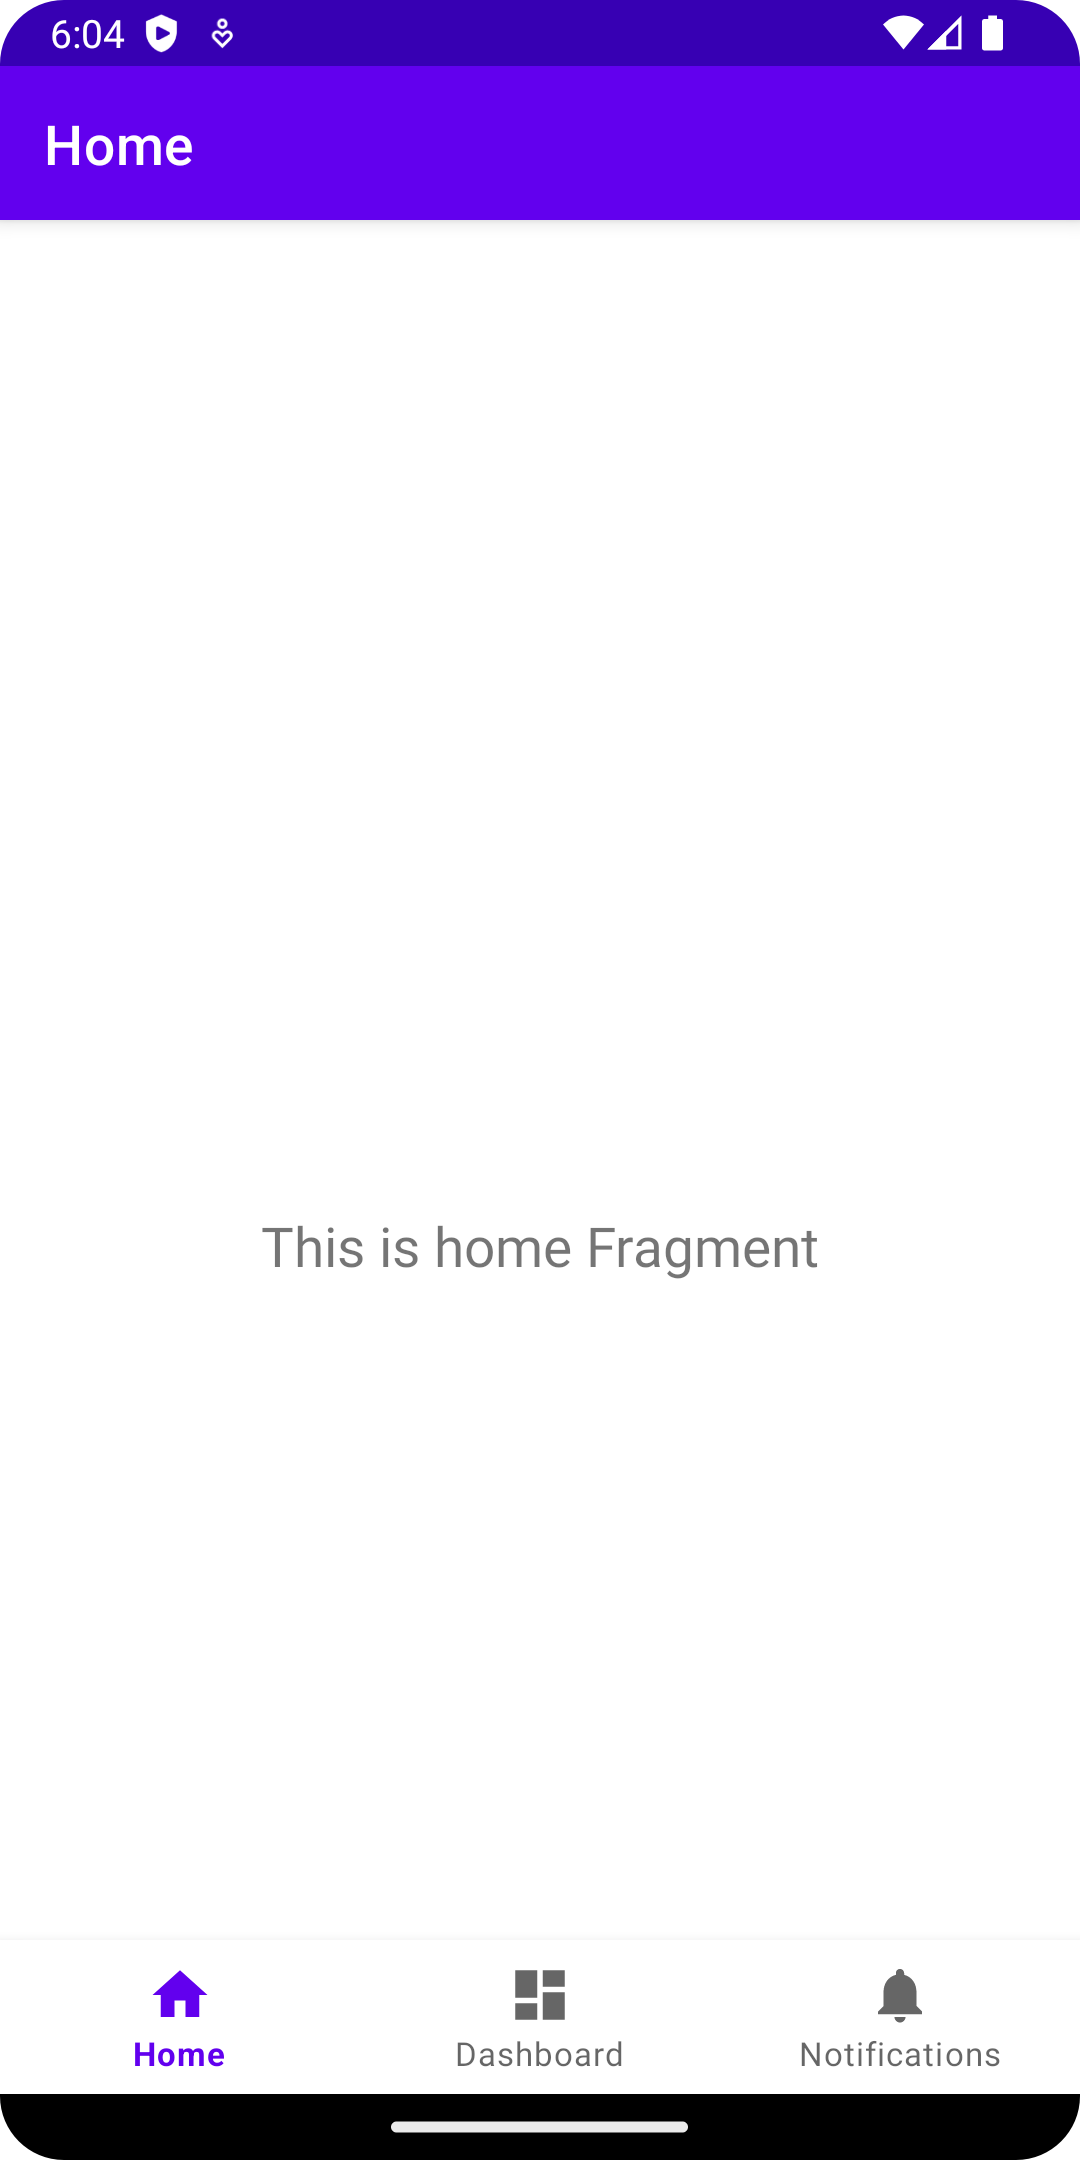
\includegraphics[height=0.4\textheight]{basis_layoutnative.png}
    \caption{Layout van applicatie voor de basisfunctionaliteiten bij Android.}
\end{figure}
